\subsection{Hadronic calorimeter}
\label{sec:hcal}

The CMS hadronic calorimeter (HCAL) 
\nomenclature{HCAL}{Hadronic calorimeter} is a hermetic sampling calorimeter 
made of alternating layers of plastic scintillator and brass absorber.
Together with the electromagnetic calorimeter (ECAL), the HCAL
forms a complete calorimetry system for the CMS detector, which
allows for the reconstruction of hadronic jets and missing transverse energy.
Like the ECAL, the HCAL is split into two subdetectors consisting 
of a barrel region (HB)
\nomenclature{HB}{Hadronic calorimeter barrel}
and two endcap regions (HE).
\nomenclature{HE}{Hadronic calorimeter endcap}
These subdetectors cover the pseudorapdity region $|\eta| < 3.0$.
The HCAL is radially restricted by the inner radius of the 
solenoid (2.95 m from the IP) and the outer radius of the ECAL
(1.77 m from the IP).  This radial restriction also restricts
the number of interaction lengths of material within the HCAL.
Therefore, an additional layer of scintillator known as the 
outer hadronic calorimeter (HO)
\nomenclature{HO}{Hadronic calorimeter outer}
is placed outside 
the solenoid in the barrel region
to serve as a ``tail catcher.'' 
In addition, forward hadronic calorimeters (HF)
\nomenclature{HF}{Hadronic calorimeter forward}
made of radiation-hard quartz fiber and steel absorber are
placed 11.2 m from the IP in the pseudorapidity
region $3 < |\eta| < 5.2$.
A schematic of the HCAL is shown in Figure \ref{fig:hcal}.

\begin{figure}
  \centering
  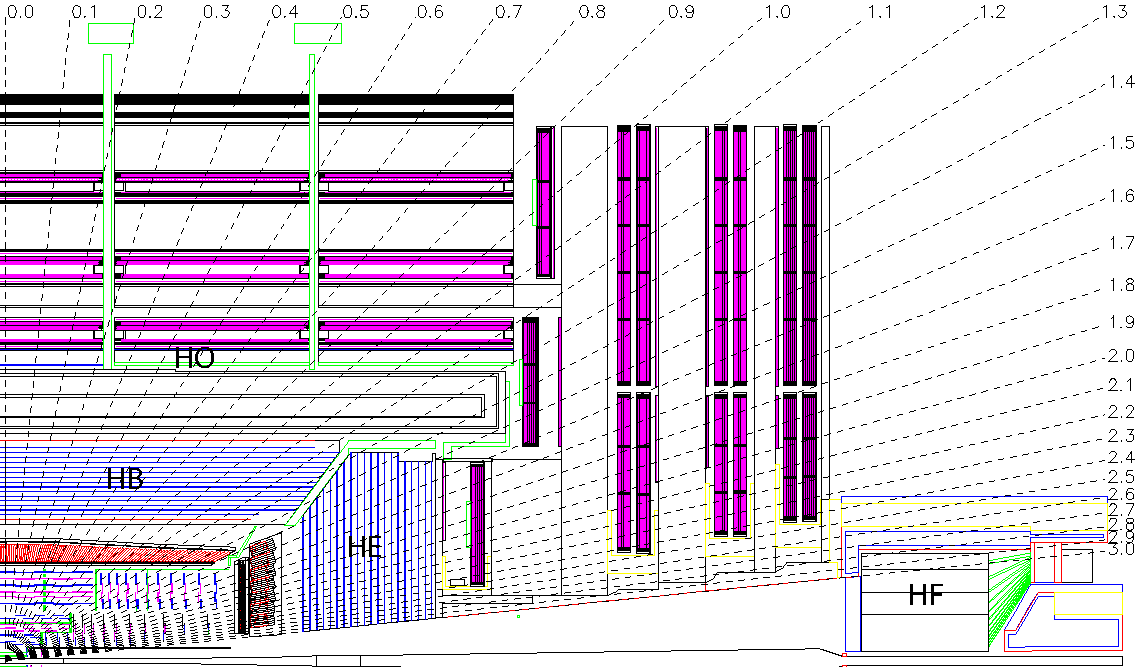
\includegraphics[width=1.0\textwidth]{tex/cms/fig/hcal-schematic.pdf}
  \caption{A schematic cross section of the CMS HCAL.  Only one quarter of the entire
    HCAL is represented. The four subsystems of the HCAL: the barrel (HB), endcap (HE),
    outer calorimeter (HO), and forward calorimeter (HF) are all shown \cite{cms-jinst}.}
  \label{fig:hcal}
\end{figure}

In order to minimize non-Gaussian tails in the energy resolution,
the HCAL must be hermetic and provide good containment of hadronic 
showers. Hence, the HB and HE absorber has been chosen to maximize the number 
of interaction lengths of material within the CMS solenoid.
C26000 ``cartridge brass'' not only satisfies this requirement, it is also nonmagnetic
and composed of relatively low-$Z$ elements (zinc and copper), which
means that it will not significantly degrade the muon measurement.
Some properties of C26000 brass are shown in Table \ref{tab:hcal-brass}.

\begin{table}
  \centering
  \begin{tabular}{c|c}
    Property & Value \\
    \hline\hline
    Chemical composition & 70\% Cu, 30\% Zn \\
    Density & 8.53 $\text{g}/\text{cm}^{3}$ \\
    Radiation length & 1.49 cm \\
    Interaction length & 16.42 cm \\
  \end{tabular}
  \caption{Properties of the HB and HE brass absorber: C26000 or ``cartridge brass'' \cite{cms-jinst}.}
  \label{tab:hcal-brass}
\end{table}

Plastic scintillator was chosen as the active medium for the HB and HE 
in part for its minimal thickness, which allowed more material 
budget to be given to the absorber.  
The plastic scintillators are
composed of tiles embedded with wavelength-shifting (WLS)
\nomenclature{WLS}{Wavelength shifting fibers}
fibers, which are spliced to high attenuation-length clear
plastic fibers that carry the light to the readout electronics.
The single innermost plastic scintillator layer of the HB and HE 
is made of Bicron BC408.  This layer samples hadronic showers 
that begin within the inert material between the ECAL and the HCAL.
All other plastic scintillator layers in both
detectors are made from Kuraray SCSN81.

\begin{figure}
  \centering
  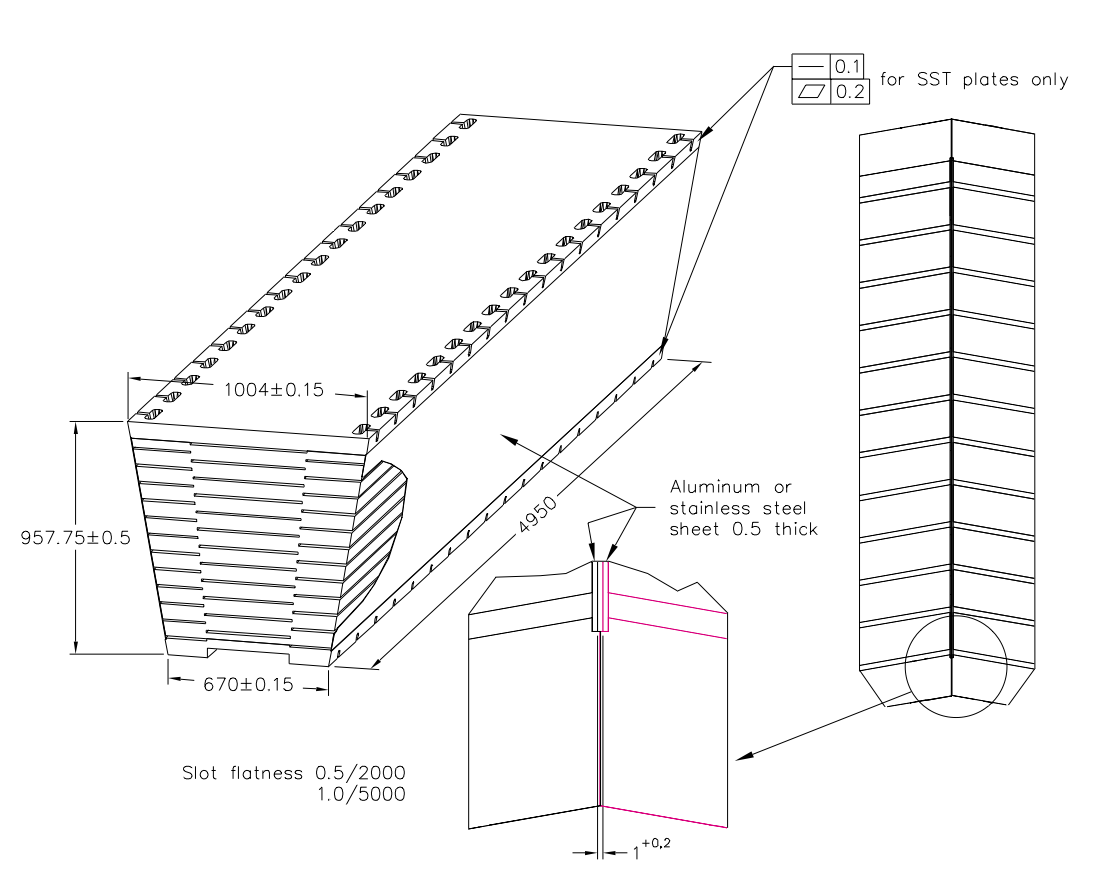
\includegraphics[width=0.7\textwidth]{tex/cms/fig/hcal-wedge.png}
  \caption{A schematic of an HB wedge showing the pattern with which the 
    absorber plates are bolted together to ensure hermiticity.  SST refers
    to the stainless steel plates at the top and bottom of each wedge \cite{cms-jinst}.}
  \label{fig:hcal-wedge}
\end{figure}

The HB covers the pseudorapidity region of $|\eta| < 1.4$.
It is composed of 36 identical azimuthal wedges, which 
form two half-barrels (HB+ and HB-).  
Each wedge is separated into 16 towers in $\eta$ and 4 towers
in $\phi$.  This makes a total of 2304 towers in the HB, each
of which covers $\Delta\eta\times\Delta\phi = 0.087\times5^{\circ}$.
These wedges are composed of flat absorber plates that have been bolted together in layers with a staggered
geometry so that there are no gaps with projective dead material, as shown in Figure \ref{fig:hcal-wedge}.
The innermost and outermost absorber layers are made of stainless steel for structural
strength; all other layers are made of brass.  The innermost stainless steel layer has a thickness
of 40 mm.  The outermost stainless steel layer has a thickness of 75 mm.  The innermost
8 brass layers have a thickness of 50.5 mm, and the outermost 14 layers have a thickness
of 56.6 mm.  The plates are bolted together in such a way as to leave
slots for plastic scintillator between them.
All of the scintillator for a given layer is grouped together into a single mechanical tray 
in order to reduce the number of mechanical components to be handled.
Each scintillator tile is 3.7 mm thick, except for the innermost and outermost tiles, which are 9 mm thick.
A single WLS fiber is embedded in each tray, which interfaces 
with a clear plastic fiber, which in turn interfaces with an optical cable.
The optical cable carries light from the scintillators to an optical decoding unit, 
which collects the fibers into read-out towers and brings the light 
to a hybrid photodiode (HPD) \nomenclature{HPD}{Hybrid photodiode}.
Each wedge has four HPDs (one for each $\phi$ segmentation), which are located
in a readout box (RBX) \nomenclature{RBX}{Readout box} on the side of the wedge 
farthest from the IP.  All scintillator layers for a single tower 
are combined into a single longitudinal readout, except in the case of 
towers 15 and 16 in the most forward region of the HB.  A schematic of the HCAL
longitudinal segmentation can be seen in Figure \ref{fig:hcal-segmentation}.
The material budget of the absorber is less than 6 interaction lengths at 
$|\eta| = 0$ and about 10 interaction lengths at $|\eta| = 1.3$. The ECAL
adds about 1.1 interaction lengths to this.

\begin{figure}
  \centering
  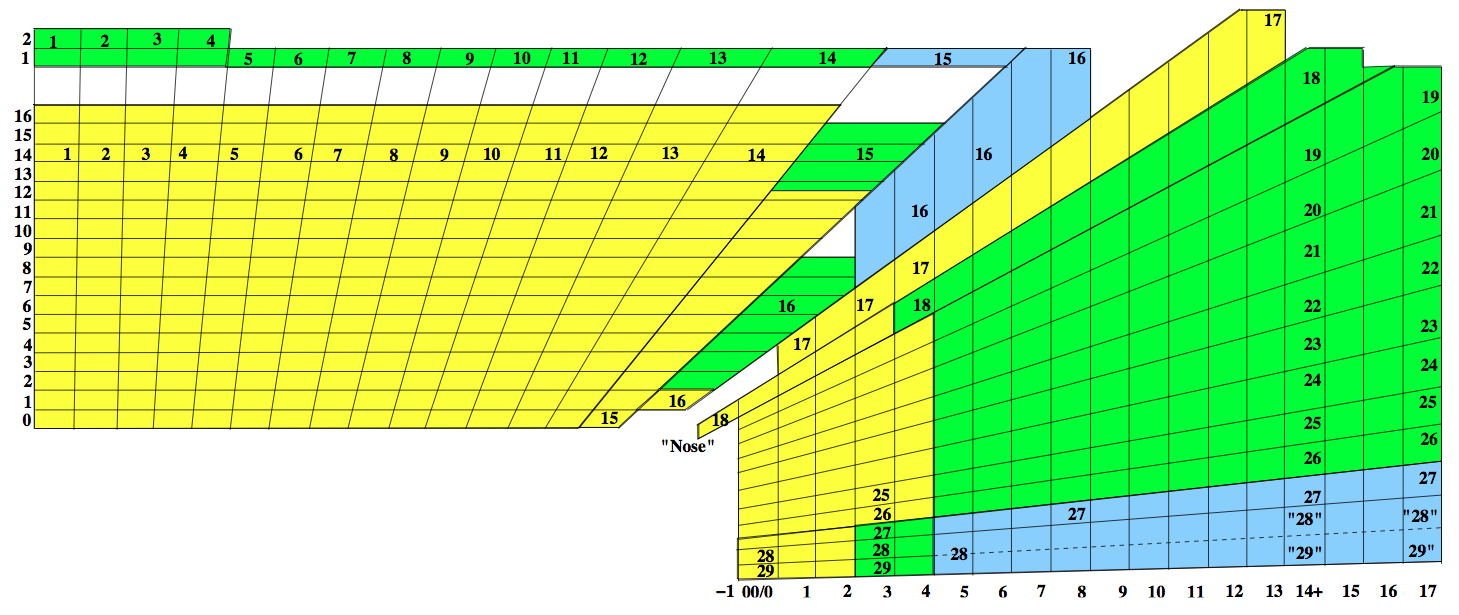
\includegraphics[width=0.95\textwidth]{tex/cms/fig/hcal-segmentation.png}
  \caption{A schematic of the CMS HCAL showing the longitudinal depth
    segmentation of the tower readout.  Only one fourth of the detector is shown.
    Each number outside the colored region on the white edge of the schematic corresponds to a 
    scintillator layer.  Each number within the colored area corresponds to a tower.  
    Each tower is read out with either one longitudinal segmentation (only yellow),
    two longitudinal segmentations (yellow and green), or three longitudinal 
    segmentations (yellow, green, and blue) \cite{hcal-geometry}.}   
  \label{fig:hcal-segmentation}
\end{figure}

The HE covers the pseudorapidity region of $1.3 < |\eta| < 3.0$.
It is designed to interlock neatly with the HB.
There are a total of 1368 towers in the HE, and the five most 
central of these towers each covers $\Delta\eta\times\Delta\phi = 0.087\times5^{\circ}$.
The rest of the HE towers vary in $\Delta\eta\times\Delta\phi$ coverage, as shown
in Table \ref{tab:hcal-segmentation}.
The HB and the HE are very similar in design.  
Like the HB, the HE is made of 
interlocking C26000 brass absorber plates with
plastic scintillator tiles that have been stacked to avoid
projective dead material.  
Also like the HB, the outermost absorber layer is made of stainless steel
rather than brass (the innermost layers are brass in the case of the HE, unlike the HB).
In the case of the HE, the absorbers are 79 mm thick.
In addition, the HE also uses WLS fibers, clear plastic fibers, and 
optical cable to route light from the plastic scintillators to an optical 
decoding unit, and HPDs within an RBX are used as the photodetectors.
The total length of the HE, including the ECAL, is about 10 interaction lengths.

\begin{table}
  \centering
  % \footnotesize
  \small
  \begin{tabular}{r|c|c|cc|c|c|cc}
    Tower & \multicolumn{2}{c|}{$\eta$ range} & \multicolumn{2}{c|}{\multirow{2}{*}{Detector}} & \multicolumn{2}{c|}{Size} & \multicolumn{2}{c}{Depth} \\ 
    index & \multicolumn{1}{c}{Low} & High & & & \multicolumn{1}{c}{$\Delta\eta$} & $\Delta\phi$ & \multicolumn{2}{c}{segments} \\ 
    \hline\hline
    1  & 0.000 & 0.087 & HB, & HO & 0.087 & $5^{\circ}$  & $\text{HB} = 1$, & $\text{HO} = 1$ \\
    2  & 0.087 & 0.174 & HB, & HO & 0.087 & $5^{\circ}$  & $\text{HB} = 1$, & $\text{HO} = 1$ \\
    3  & 0.174 & 0.261 & HB, & HO & 0.087 & $5^{\circ}$  & $\text{HB} = 1$, & $\text{HO} = 1$ \\
    4  & 0.261 & 0.348 & HB, & HO & 0.087 & $5^{\circ}$  & $\text{HB} = 1$, & $\text{HO} = 1$ \\
    5  & 0.348 & 0.435 & HB, & HO & 0.087 & $5^{\circ}$  & $\text{HB} = 1$, & $\text{HO} = 1$ \\
    6  & 0.435 & 0.522 & HB, & HO & 0.087 & $5^{\circ}$  & $\text{HB} = 1$, & $\text{HO} = 1$ \\
    7  & 0.522 & 0.609 & HB, & HO & 0.087 & $5^{\circ}$  & $\text{HB} = 1$, & $\text{HO} = 1$ \\
    8  & 0.609 & 0.696 & HB, & HO & 0.087 & $5^{\circ}$  & $\text{HB} = 1$, & $\text{HO} = 1$ \\
    9  & 0.696 & 0.783 & HB, & HO & 0.087 & $5^{\circ}$  & $\text{HB} = 1$, & $\text{HO} = 1$ \\
    10 & 0.783 & 0.879 & HB, & HO & 0.087 & $5^{\circ}$  & $\text{HB} = 1$, & $\text{HO} = 1$ \\
    11 & 0.879 & 0.957 & HB, & HO & 0.087 & $5^{\circ}$  & $\text{HB} = 1$, & $\text{HO} = 1$ \\
    12 & 0.957 & 1.044 & HB, & HO & 0.087 & $5^{\circ}$  & $\text{HB} = 1$, & $\text{HO} = 1$ \\
    13 & 1.044 & 1.131 & HB, & HO & 0.087 & $5^{\circ}$  & $\text{HB} = 1$, & $\text{HO} = 1$ \\
    14 & 1.131 & 1.218 & HB, & HO & 0.087 & $5^{\circ}$  & $\text{HB} = 1$, & $\text{HO} = 1$ \\
    15 & 1.218 & 1.305 & HB, & HO & 0.087 & $5^{\circ}$  & $\text{HB} = 2$, & $\text{HO} = 1$ \\
    16 & 1.305 & 1.392 & HB, & HE & 0.087 & $5^{\circ}$  & $\text{HB} = 2$, & $\text{HE} = 1$ \\
    17 & 1.392 & 1.479 & HE  &    & 0.087 & $5^{\circ}$  & $\text{HE} = 1$  & \\
    18 & 1.479 & 1.566 & HE  &    & 0.087 & $5^{\circ}$  & $\text{HE} = 2$  & \\
    19 & 1.566 & 1.653 & HE  &    & 0.087 & $5^{\circ}$  & $\text{HE} = 2$  & \\
    20 & 1.653 & 1.740 & HE  &    & 0.087 & $5^{\circ}$  & $\text{HE} = 2$  & \\
    21 & 1.740 & 1.830 & HE  &    & 0.090 & $10^{\circ}$ & $\text{HE} = 2$  & \\
    22 & 1.830 & 1.930 & HE  &    & 0.100 & $10^{\circ}$ & $\text{HE} = 2$  & \\
    23 & 1.930 & 2.043 & HE  &    & 0.113 & $10^{\circ}$ & $\text{HE} = 2$  & \\
    24 & 2.043 & 2.172 & HE  &    & 0.129 & $10^{\circ}$ & $\text{HE} = 2$  & \\
    25 & 2.172 & 2.322 & HE  &    & 0.150 & $10^{\circ}$ & $\text{HE} = 2$  & \\
    26 & 2.322 & 2.500 & HE  &    & 0.178 & $10^{\circ}$ & $\text{HE} = 2$  & \\
    27 & 2.500 & 2.650 & HE  &    & 0.150 & $10^{\circ}$ & $\text{HE} = 3$  & \\
   *28 & 2.650 & 3.000 & HE  &    & 0.350 & $10^{\circ}$ & $\text{HE} = 3$  & \\
    29 & 2.853 & 2.964 & HF  &    & 0.111 & $10^{\circ}$ & $\text{HF} = 2$  & \\
    30 & 2.964 & 3.139 & HF  &    & 0.175 & $10^{\circ}$ & $\text{HF} = 2$  & \\
    31 & 3.139 & 3.314 & HF  &    & 0.175 & $10^{\circ}$ & $\text{HF} = 2$  & \\
    32 & 3.314 & 3.489 & HF  &    & 0.175 & $10^{\circ}$ & $\text{HF} = 2$  & \\
    33 & 3.489 & 3.664 & HF  &    & 0.175 & $10^{\circ}$ & $\text{HF} = 2$  & \\
    34 & 3.664 & 3.839 & HF  &    & 0.175 & $10^{\circ}$ & $\text{HF} = 2$  & \\
    35 & 3.839 & 4.013 & HF  &    & 0.174 & $10^{\circ}$ & $\text{HF} = 2$  & \\
    36 & 4.013 & 4.191 & HF  &    & 0.178 & $10^{\circ}$ & $\text{HF} = 2$  & \\
    37 & 4.191 & 4.363 & HF  &    & 0.172 & $10^{\circ}$ & $\text{HF} = 2$  & \\
    38 & 4.363 & 4.538 & HF  &    & 0.175 & $10^{\circ}$ & $\text{HF} = 2$  & \\
    39 & 4.538 & 4.716 & HF  &    & 0.178 & $10^{\circ}$ & $\text{HF} = 2$  & \\
    40 & 4.716 & 4.889 & HF  &    & 0.173 & $20^{\circ}$ & $\text{HF} = 2$  & \\
    41 & 4.889 & 5.191 & HF  &    & 0.302 & $20^{\circ}$ & $\text{HF} = 2$  & \\
  \end{tabular}
  \caption{Table showing the segmentation of the CMS HCAL.
    The pseudorapidity range, detector, coverage in $\Delta\eta\times\Delta\phi$,
    and longitudinal depth segmentation details are all shown. Longitudinal 
depth segmentation can also be seen in Figure \ref{fig:hcal-segmentation} \cite{hcal-geometry}. \\ 
    * The first two depth segmentations have finer $\eta$ segmentation, namely 
    $2.650-2.868$ and $2.868-3.000$ and are referred to as tower indices 28 and 29.}
  \label{tab:hcal-segmentation}
\end{table}  

The HO covers the pseudorapidity region of $|\eta| < 1.26$.
Unlike the HB and HE subdetectors, the HO is composed 
only of scintillators and is placed outside of the solenoid bore.
At $\eta = 0$, the HB and EB together only provide about seven interaction
lengths.  The HO, therefore, is designed to sample the energy
from hadronic showers that penetrate both the HB and HE and leak out 
of the solenoid.  By using the solenoid as an additional absorber,
the HO in principle increases the effective thickness of the HCAL in 
the barrel region and reduces non-Gaussian tails in the energy
resolution.  The HO is located inside of the barrel muon system
(Section \ref{sec:muon}), and so it is spatially restricted by that system.
The HO is divided into five rings, which are labeled: -2, -1, 0, 1, and 2.
Each of these rings is divided into 12 identical $\phi$-sectors, and each $\phi$-sector
has 6 slices in $\phi$.
Ring 0 of the HO has two scintillator layers on either side of a 19.5 cm 
piece of iron at 3.82 m and 4.07 m from the IP.  The other HO rings 
have only one HO layer at a distance of 4.07 m from the IP.
Each HO layer is 40 mm thick, 16 mm of which is taken up by the scintillator,
while the rest is taken up by an aluminum honeycomb support structure, and each
ring takes up 2.54 m on the $z$-axis.
Like the HB and HE, the HO scintillator is unified in tiles, and the size 
and shape of the HO tiles roughly maps to the HB towers.
Also like the HB and HE, light from the HO scintillators is collected via
WLS fibers, clear plastic fibers, and optical cable.
HPDs within an RBX are used as the photodetectors.

The HF covers the pseudorapidity region of $3.0 < |\eta| < 5.0$ and is located
125 cm from the beam.  This region is exposed to unprecedented particle fluxes, 
and successful operation relies strongly on radiation hardness.  For this reason,
unlike the HB, HE, and HO, the HF uses steel as an absorber 
and quartz fibers as an active medium (the signal being 
Cerenkov light emitted within the quartz fibers).
In addition, light is collected using photomultiplier tubes (PMTs)
\nomenclature{PMT}{Photomultiplier tubes} rather than HPDs.
The HF is essentially cyllindrical and made up of $18\times20^{\circ}$ steel wedges on either
side of the IP.  The cyllinder's outer radius is 130 cm and the inner radius is 12.5 cm.
The steel absorber is 165cm deep, and the quartz fibers are 0.6 mm in diameter.
The fibers run parallel to the beamline, and they 
are bundled together to form a total of 864 towers (without pointing geometry).
Half of the fibers are ``long'' and run the full length of the HF detector, while
the other half are ``short'' and start 22 cm from the front face of the HF detector.
This allows for the discrimination between electromagnetic showers, which are 
generally absorbed before reaching the short fibers, and hadronic showers, 
which interact with both long and short fibers.

The HCAL energy resolution 
($\sigma/E$) for a pion of given energy $E$ may be parameterized by 
Equation \ref{eqn:hcal-resolution-1}:
\begin{equation}
  \frac{\sigma(E)}{E} =
  \frac{S}{\sqrt{E}} \oplus C 
  \label{eqn:hcal-resolution-1}
\end{equation}
where $S$ is the stochastic term and $C$ is the constant term.
These terms have been measured in test beams using a $5\times5$
HB tower array and a pion beam, and the results are given in
Equation \ref{eqn:hcal-resolution-2}:
\begin{equation}
  \frac{\sigma(E)}{E} =
  \frac{115.3\% \text{ GeV}^{1/2}}{\sqrt{E}} \oplus 5.5\%
  \label{eqn:hcal-resolution-2}
\end{equation}
The results are shown graphically in Figure \ref{fig:hcal-resolution}.
Similar results were obtained with the HF using pion and electron test beams,
where $S = 198\%$, $C = 9\%$ for electromagnetic shower energy resolution and $S = 280\%$, 
$C = 11\%$ for hadronic shower energy resolution \cite{cms-jinst,cms-tdr,hf-resolution}.

\begin{figure}
  \centering
  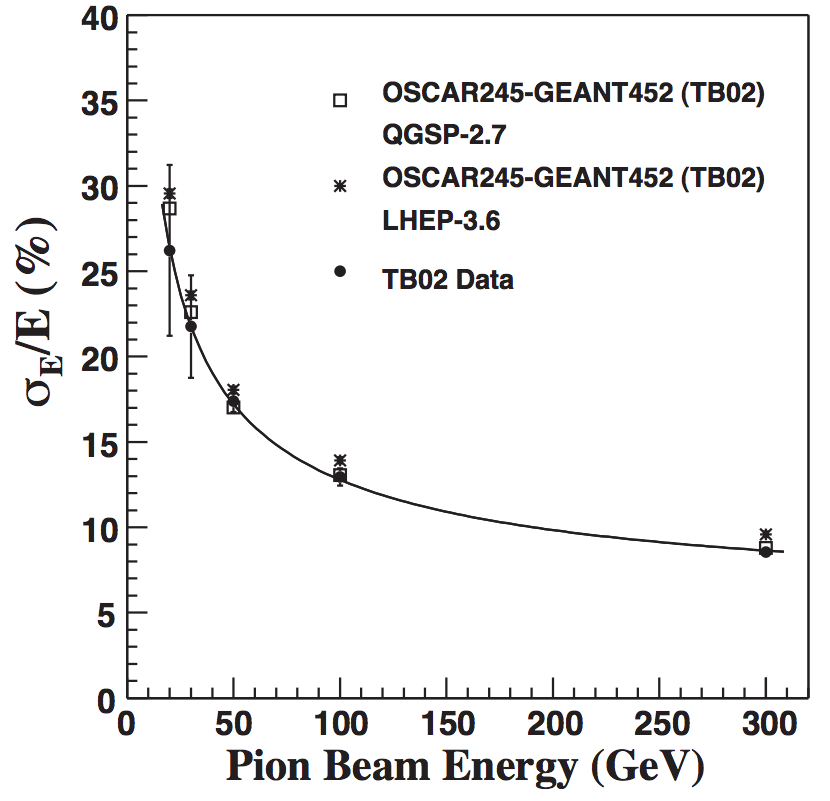
\includegraphics[width=0.6\textwidth]{tex/cms/fig/hcal-resolution.png}
  \caption{Energy resolution of the HB as a function of pion energy as measured in a test beam \cite{hcal-resolution}.}
  \label{fig:hcal-resolution}
\end{figure}


